\section{Education Variables}
\label{sec:edu}
\subsection{Maximum Education}

Maximum education variable has 9 categories, which are shown in Table \ref{tab:par-maxedu}. Since Italian education system has experienced changes in 1999 due to Bologna process\footnote{Bologna process is a series of ministerial meetings and agreements between European countries designed to ensure comparability in the standards and quality of higher education qualifications.}, those need to be accounted for when converting the education categories into years of education. Column 3 of Table \ref{tab:par-maxedu} shows the converted years of education according to information below. 

Italian elementary school (Scuola elementare) lasts 5 years. We assume that all parents for younger cohorts attended elementary school unless noted otherwise. ``Scuola media inferiore" last for 3 years (roughly from age 11 to 13). There are two types of high school listed in our category. ``Biennio scuola media superiore" offers two years of education and the ``Scoula media superiore" offers 4 or 5 years of education. 

After the Bologna agreement, most of universities in Italy became a 3+2 system, each period granting a certification. First 3 years (laurea triennale) can be considered as a bachelors, and the second 2 years (laurea biennale) can be translated as a masters program. However, in reality, 3+2 is same as previous university degree (diploma universitario). Because of the timing when this change took place, these years of education does not apply to age-40 and age-50 cohorts in the Reggio data. 

There are some difference in how degrees are called in Italy and in the United States. ``Laurea specialistica o magistrale" in our category, although it is translated as ``master", is more similar to bachelor's in the United States. On the other hand, ``master post-laurea", which includes MBA, can be considered as the actual master's degree. 


\begin{table}[H]
\caption{Categories for Parental Maximum Education} \label{tab:par-maxedu}
\begin{center}
\begin{tabular}{L{4.3cm} L{4.3cm} L{4.3cm}}
\toprule
\textbf{Italian Label} & \textbf{English Label} & \textbf{Years of Education} \\ \midrule
	(1) Scuola media inferiore/licenza elementa &	Junior High School/Primary School		& 8 years \\
	(2) Biennio scuola media superiore & 				Two years high school								& 10 years \\
	(3) Scuola media superiore (4 o 5 anni) & 		High School (4 or 5 years)								& 12 years \\
	(4) Diploma universitario &	University Diploma & 16 years \\
	(5) Laurea triennale &	Three-year Degree &	15 years \\
	(6) Laurea quadriennale/quinquennale &   	Five-year Degree & 17 years \\
	(7) Laurea specialistica o magistrale & 			Master & 17 years \\
	(8) Master post-laurea quadr./quinq./sp  & Master postgraduate framework			& 19 years \\
	(9) Dottorato di ricerca 	& Ph.D.	& 23 years \\ \bottomrule
\end{tabular}
\end{center}
\end{table}

\subsection{High School Grades}
High school grade (votoMaturita) that was asked in the questionnaires has two different scales, one has the maximum scoring of 60 and the other has 100. The former scale is the old scoring scheme that was changed to latter by the law n.1/2007. Before 2007, the maximum grade was 60 and the minimum passing grade was 36 (below 36 was fail). After 2007, the maximum grade became 100 and the minimum passing grade became 60 (below 60 is fail)\footnote{http://www.classbase.com/Countries/italy/Grading-System}.

Since adolescent cohort went to high school after the change in scoring system, the questionnaire for adolescents asks respondents to provide their high school grades in 100 scale. On the other hand, since people the adult cohorts might have used 60 scale when they attended high school, the questionnaire for adults ask respondents two different choices (old way and new way) to report their high school grade. 



\section{Cognitive Variables}
\label{sec:cog}

IQ is measured for all individuals in the sample as well as for the caregivers of the children, migrants, and adolescents using Raven's Progressive Matrices (Raven's).\footnote{\citet{Raven_Raven_etal_1988_BOOKManualRavensprogressive}.} Raven's is a non-verbal test that is correlated with other measures of fluid intelligence. The 12-Item and 18-Item versions are shortened from the original version, which helps reduce the duration of the test. Both shortened versions are highly correlated with the full version of the test, which in turn is highly correlated with other measures of IQ.

Each item on the test consists of a matrix of diagrams that follow some logical pattern with one missing diagram that the test-taker needs to select from multiple choices. A correct answer is assigned a value of 1, and an incorrect answer is assigned a value of 0. The IQ score is the proportion of questions answered correctly. If questions are missed, then they do not count in the total number of questions. The factor scores are computed using a specification of a structural equation using maximum likelihood that accounts for missing values. That is, it requires the assumption that bot the observed and latent variables are jointly distributed normally, and that any missing values are missing at random. The latter assumption is the more tenuous assumption given that a missing item could mean the individual could not answer the question at all due to lower cognitive ability (as opposed to rushing through the test or inability to focus).
% The variables that measure these binary item-level responses for subjects are IQ*. For caregivers, the analogous variables are cgIQ*.

 Table \ref{tab:test-type} explains which individuals in which cohort received the 12- or 18-Item version of Raven's Progress Matrices (Raven's).

\begin{table}[H]
\begin{center}
	\caption{IQ Test by Cohort}\label{tab:test-type}
	\begin{tabular}{lcc}
		\toprule
		Cohort & 12-Item & 18-Item \\
		\midrule
		\textbf{Children} & &\\
		\quad Subjects & & $\checkmark$  \\
		\quad Caregivers &  $\checkmark$ & \\
		\textbf{Migrants} & & \\
		\quad Subjects & & $\checkmark$ \\
		\quad Caregivers & $\checkmark$ &  \\
		\textbf{Adolescents} & & \\
		\quad Subjects & $\checkmark$ & \\
		\quad Caregivers &  $\checkmark$ &  \\
		\textbf{Adults} & & \\
		\quad Subjects & & $\checkmark$ \\
		\bottomrule
	\end{tabular}
\end{center}
\raggedright \footnotesize Note: This table shows the type of test given for each cohort. The caregivers were always given the 12-Item Raven's. The 18-Item Raven's was only meant for younger subjects (the individuals in the children and migrants cohorts were about 6 years old at the time of the test).
\end{table}

Figure \ref{fig:iq-hist} shows the distribution of the IQ score by city and cohort. 

\begin{figure}[H]
	\begin{center}
	\caption{Densities of IQ Scores}\label{fig:iq-hist}
	\begin{subfigure}{.5\textwidth}
		\centering
		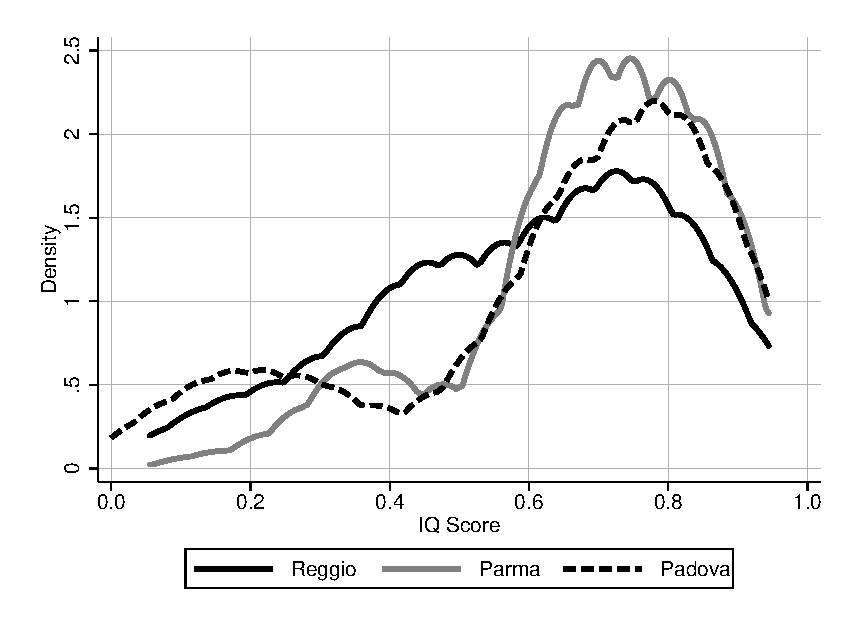
\includegraphics[width=20em]{../../../../Output/IQ_hist_1}
		\caption{Children}
	\end{subfigure}%
	\begin{subfigure}{.5\textwidth}
		\centering
		\includegraphics[width=20em]{../../../../Output/IQ_hist_2}
		\caption{Migrants}
	\end{subfigure}
	\begin{subfigure}{.5\textwidth}
		\centering
		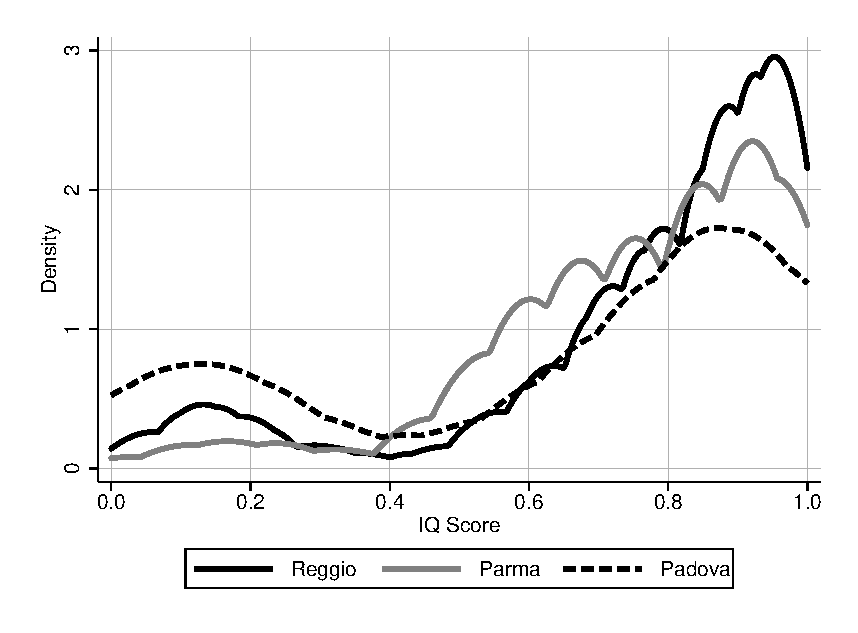
\includegraphics[width=20em]{../../../../Output/IQ_hist_3}
		\caption{Adolescents}
	\end{subfigure}%
	\begin{subfigure}{.5\textwidth}
		\centering
		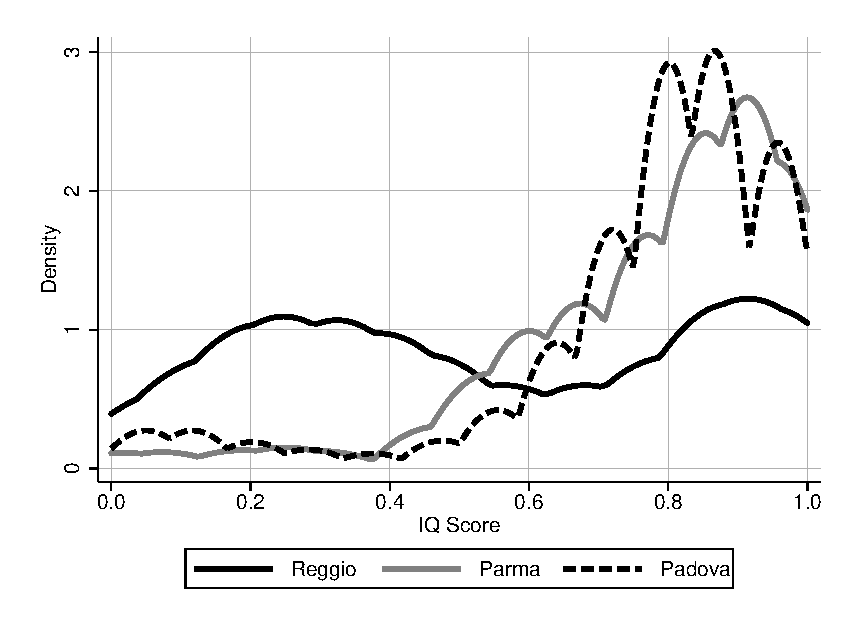
\includegraphics[width=20em]{../../../../Output/IQ_hist_4}
		\caption{Adults 30s}
	\end{subfigure}
	\begin{subfigure}{.5\textwidth}
		\centering
		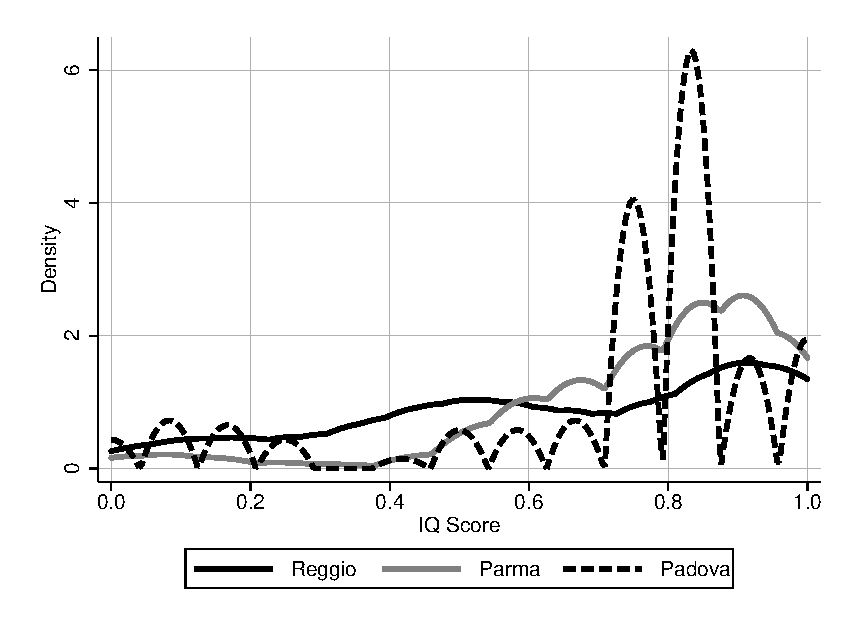
\includegraphics[width=20em]{../../../../Output/IQ_hist_5}
		\caption{Adults 40s}
	\end{subfigure}%
	\begin{subfigure}{.5\textwidth}
		\centering
		\includegraphics[width=20em]{../../../../Output/IQ_hist_6}
		\caption{Adults 50s}
	\end{subfigure}
\end{center}
\raggedright \footnotesize
Note: These plots show the distributions of IQ scores by city and cohort. The distributions of the different cities are more similar for the younger cohorts than for the adult cohorts. 
\end{figure}


\section{Income and Employment Variables}
\label{sec:income}
\subsection{Family Income}

Table \ref{tab:faminc} lists categories of income in our questionnaire. This category is used for (i) baseline family income and (ii) current family income. Although (i) and (ii) are measuring income at different point of time with different inflation rates, since the questions that were asked does not account for the inflation rate, we do not account for inflation rate when converting categories into values. We apply median of reported category when creating income variables shown in values. 

\begin{table}[H]
\caption{Categories for Family Income} \label{tab:faminc}
\begin{center}
\begin{tabular}{ll}
\toprule
\textbf{Category} & \textbf{Value} \\ \midrule
	1 - 5,000 Euro					 & 2,500 Euro \\
	5,001 - 10,000 Euro				 & 7,500 Euro \\
	10,001 - 25,000 Euro			 & 17,500 Euro \\
	25,001 - 50,000 Euro			 & 37,500 Euro \\
	50,001 - 100,000 Euro			 & 75,000 Euro \\
	100,001 - 250,000 Euro			 & 175,000 Euro \\
	More than 250,000 Euro			 & 375,000 Euro \\ \bottomrule
\end{tabular}
\end{center}
\end{table}
	
\subsection{Caregiver's Occupation and Hours of Work}
Caregiver's occupation variable has 12 categories in the questionnaire: (i) never worked, (ii) farmer, (iii) worker, (iv) employee, (v) teacher, (vi) executive, (vii) manager, (viii) professional (doctor, lawyer, etc.), (ix) entrepreneur, (x) self-employed, (xi) atypical worker, (xii) other.  

There are two measures of caregiver's hours of work in the questionnaire: (i) normal hours of work per week and (ii) average overtime hours per week. Caregiver's total hours of work per week is computed by combining normal hours and overtime hours. Moreover, if a caregiver reported to have ``never worked" when reporting occupation, we record the total hours of work for such caregiver as 0 hours. The mean total hours of work of caregiver is  34.57 hours with the standard error 12.99. The minimum weekly hours of worked is 0 hour and the maximum is 90 hours in the data.

\subsection{House Ownership}
The question that asks "Is this house owned by this household?" is both for parents of children and adolescents and for adults. This means that for younger cohorts, this variable shows the ownership of their caregivers. For adult cohorts, this variable shows whether respondent owns house. 
